\begin{frame}
\label{frame:wfd_complexity_details}
\frametitle{\WFD Best Case}
\begin{itemize}
\item Notation:
	\begin{itemize}
	  \item $S_{open}:=$ the area of the shape 
	  \item $P_{opt}:=$ the perimeter of the shape
	\end{itemize}
\item The best case holds:
\end{itemize}
$$
S_{open} = 4\pi r^2
$$
$$
P_{opt} = 2\pi r
$$
\end{frame}

\begin{frame}
\frametitle{\WFD Worst Case}
\begin{columns}
\column{0.7\textwidth}
Notation (for a given $k$ vertices):
\begin{itemize}
  \item $S_k:=$ the area of the shape.
  	\begin{itemize}
  	  \item $S_k = S_{open}$ (area remains the same)
  	\end{itemize}
  \item $P_k:=$ the perimeter of the shape.
  \item $b_k:=$ the base of the inner \openspace polygon.
  \item $h_k:=$ the height of an outer triangle
  \item $l_k:=$ the length of an outer triangle side.
\end{itemize}
\column{0.3\textwidth}
\def\MyTikzScale{1.5}
\def\bgColor{gray!15}

\def\createBackground{% The graphic
  \draw[fill=\bgColor] (-1.2,-1.2) -- (1.2,-1.2) -- (1.2,1.2) -- (-1.2,1.2) --
  (-1.2,-1.2);
 }


\definecolor{myColor}{RGB}{94,38,18}
\def\emphColor{myColor}
\def\arrowWidth{1pt}
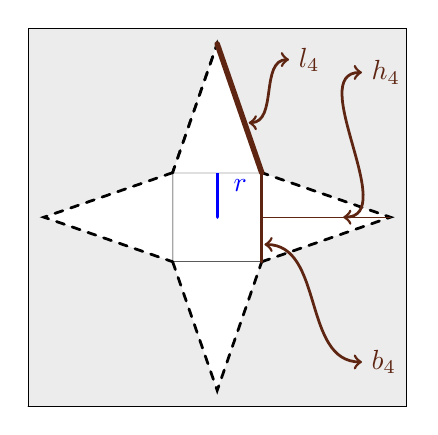
\begin{tikzpicture}[scale=\MyTikzScale,cap=round]
  % Local definitions
  \def\costhirty{0.8660256}
  \def\cosforthyfive{0.7071067811}
  % Colors
  \colorlet{coscolor}{blue}

  % Styles
  \tikzstyle{axes}=[]
  \tikzstyle{important line}=[very thick]
  %\tikzstyle{information text}=[rounded corners,fill=red!10,inner sep=1ex]

  \createBackground
    
%     \path (-0.2,-0.2) coordinate (A) (0.2,-0.2) coordinate (B)
%           (0.2,0.2) coordinate (C) (-0.2,0.2) coordinate (D);
%         \draw[fill=white] (A)--(B)--(C)--(D)--cycle;
        
    \newdimen \R
    \R=0.4cm
     \draw[fill=white] (45:\R) \foreach \x in {0,45,135,...,405} {
     	-- (\x:\R)
     } -- cycle (135:\R);

   \draw[style=important line,coscolor]
    (0,0) -- node[right=2pt,fill=none] {$r$}
    (90:\R);
    
    
    
    
    \foreach \x in {45,135,...,405} {
%  		\prev=67.5;
     	\path (\x:\R) coordinate (P1) ;
     	\path (45+\x:\R+0.7cm) coordinate (P2);
     	\path (90+\x:\R) coordinate (P3);
     	\draw[fill=white, dashed, line width=1pt] (P1) -- (P2) -- (P3);
    }
% 	\draw[fill=white] (22.5:\R) \foreach \x in {67.5,112.5,...,382.5} {
%      	-- (\x:\R)
%      }	
    
    %\draw[fill=white, line width=1pt,dashed] (A)--(0,-1.2)--(B);
    %\draw[fill=white] (B)--(BC)--(C)--cycle;
    %\draw[fill=white] (C)--(CD)--(D)--cycle;
    %\draw[fill=white] (D)--(DA)--(A)--cycle;

    \draw[style=important line,\emphColor]
    (-45:\R) -- node[left=0pt,fill=none] {}
    (45:\R);
    
    \draw[\emphColor]
    (\R-0.11cm,0) -- node[left=5pt,above=0pt,fill=none] {}
    (0.7cm+\R,0);
    
    \node[anchor=east] at (\R+\R,0) (src_h) {};
  	\node[color=\emphColor,anchor=west] at (45:1.3cm) (dst_h) {$h_{4}$};
  	\node[anchor=east] at (-30:0.866*\R) (src_b) {};
  	\node[color=\emphColor,anchor=west] at (-45:1.3cm) (dst_b) {$b_{4}$};
  	\draw[\emphColor,line width=\arrowWidth] (dst_h) edge[out=180,in=0,<->]
  	(src_h); 
  	\draw[\emphColor,line width=\arrowWidth] (dst_b) edge[out=180,in=0,<->]
  	(src_b);
  	
  	\node[anchor=east] at (\R*0.5,1.5*\R) (src_l) {};
  	\node[color=\emphColor,anchor=west] at (65.5:1.1cm) (dst_l) {$l_{4}$};
  	\draw[\emphColor,line width=\arrowWidth] (dst_l) edge[out=180,in=0,<->]
  	(src_l); \draw[fill=white, \emphColor,line width=2pt] (P1) -- (P2); %l4
  	
%     \draw[style=important line,red]
%     (0.3cm,0) -- node[left=5pt,above=0pt,fill=none] {$h_4$}
%     (2.6*\R,0);
    
\end{tikzpicture}
\def\MyTikzScale{2}
\end{columns}
\end{frame}


\begin{frame}
\frametitle{\WFD Worst Case}
\only<+>{
\begin{itemize}
  \item The \openspace regions are equal: 
\begin{eqnarray}\label{eq:h_k}
S_k &=& S_{open} \nonumber\\
\underbrace{k\cdot\frac{r\cdot b_k}{2}}_{\text{inner polygon}} +
\underbrace{k\cdot\frac{h_k\cdot b_k}{2}}_{\text{outer triangles}} &=& 4\pi r^2
\nonumber
\end{eqnarray}

  \item We can express $b_k$ by:

\begin{equation}\label{eq:b_k}
b_k = 2r\cdot\tan{\frac{\pi}{k}}\nonumber
\end{equation}

  \item $\Rightarrow$ $h_k$ can be expressed by:

\begin{equation}
h_k = \frac{8\pi r^2}{k\cdot b_k} - r\nonumber
\end{equation}

\end{itemize}
}

\only<+>{
\begin{itemize}
  \item Each outside triangle edge can be expressed by:
  	$$l_k = \sqrt{\term{h_k}^2 + \term{\frac{b_k}{2}}^2}$$
  \item The length of the polygon perimeter equals to:
    $$P_k = 2k\cdot l_k$$
  \item We would like to express $P_k$ as a function of $S_{open}$:
  	$$P_k = \sqrt{\term{\frac{2\cdot S_{open}}{r\cdot\tan{\frac{\pi}{k}}}}^2
	       -8\frac{k\cdot S_{open}}{\tan{\frac{\pi}{k}}}
	       + 4\frac{k^2\cdot r^2}{\cos^2{\frac{\pi}{k}}}}$$ 
\end{itemize}
}

\only<+>{
\begin{itemize}
  \item Since $k \le S_{open}$, $P_k$ can be bounded by:
	$$P_k \le \sqrt{\term{\frac{2\cdot S_{open}}{r\cdot\tan{\frac{\pi}{S_{open}}}}}^2
	       -8\frac{S_{open}^2}{\tan{\frac{\pi}{S_{open}}}}
	       + 2\cdot S_{open}^2\cdot r^2}$$
  \item $\Rightarrow$ Run-time complexity of \WFD in terms of \openspace
  area: 
  
  %\item \alert{XXX: do we need to add a supproting graph?}
\end{itemize}

$$
  \order{S_{open} +
\sqrt{\term{\frac{
S_{open}}{r\cdot\tan{\frac{\pi}{S_{open}}}}}^2
-\frac{S_{open}^2}{\tan{\frac{\pi}{S_{open}}}} + S_{open}^2\cdot r^2
	 }
}
  $$
  \hyperlink{frame:wfd_complexity}{\beamergotobutton{Back to Slide}}
}

\end{frame}